% Generated by tools/docx_tex.py from v2_1.docx. The .docx is the layout master;
% this file holds the text. Build the .docx with: docx_tex.py build <base.docx> <this.tex> <out.docx>
\documentclass[12pt]{article}
\usepackage{fontspec}\setmainfont{Liberation Serif}
\usepackage[russian]{babel}\usepackage[margin=2.5cm]{geometry}\usepackage{graphicx}
\begin{document}

% @p 0
УДК 621.3962.3.5. Математическое и программное обеспечение вычислительных систем, комплексов и компьютерных сетей

% @p 1
DOI

% @p 2
\subsection*{Подход к валидации автоматных спецификаций на основе перемножения вложенных автоматов}

% @p 3
В. А. Назарова, Бакалавр прикладной математики и информатики, orcid.org/0009-0000-0352-7885, nazarov.vladimir.a@gmail.comА. А. Шалыто, Докт. техн. наук, Профессор, orcid.org/0000-0002-2723-2077

% @p 4
аСанкт-Петербургский национальный исследовательский университет информационных технологий, механики и оптики, Кронверкский пр., 49, Санкт-Петербург, 197101, РФ

% @p 5
Введение: … Цель: … Методы: … Результаты: предлагаемый: … Практическая значимость: … Обсуждение: …

% @p 6
Ключевые слова – автоматы, вложенные автоматы, перемножение автоматов, валидация.

% @p 33
UDC 621.396

% @p 34
DOI

% @p 35
\subsection*{An approach to validating automaton specifications based on the product of nested automata}

% @p 36
V. A. Nazarova, Bachelor of science in applied mathematics and informatics, orcid.org/0009-0000-0352-7885, nazarov.vladimir.a@gmail.comA. A. Shalyto, Dr. Sc., Tech, Professor, orcid.org/0000-0002-2723-2077

% @p 37
aSaint Petersburg National Research University of Information Technologies, Mechanics and Optics, 49 Kronverksky Ave., 197101 St. Petersburg, Russian Federation

% @p 38
Introduction: ... Purpose: ... Methods: ... Results: ... Practical relevance: ... Discussion: ...

% @p 39
Keywords – automata, nested automata, automata composition, validation.

% @p 43
\subsection*{Введение}

% @p 44
В предыдущей работе [1] был предложен подход к валидации автоматных спецификаций, основанный на перемножении автоматов. Новизна подхода состояла в перемножении вложенных автоматов – автоматов, размещенных в состояниях других автоматов. Подход был продемонстрирован на системе «игровой автомат» [x] из трёх взаимосвязанных автоматов: «Игровая машина» ($A_{0}$), «Монетоприемник» ($A_{1}$) и «Игровые барабаны» ($A_{2}$). В этой системе автомат $A_{2}$ вложен в состояние «Игра» автомата $A_{0}$. Однако у подхода было три ограничения:
% @comment: Замечание 1.0: ссылка на предыдущую работу – [1], источник добавлен в раздел «Литература» в конце. Второе [x] («игровой автомат» [x]) оставлено: это ссылка на источник самой системы (в работе [1] это [29] «Имитатор игрового автомата класса „Однорукий бандит“»), его нужно добавить в литературу вторым номером.

\begin{enumerate}
% @p 45
\item В состояние мог быть вложен только один автомат.
% @p 46
\item Автомат мог быть вложен только в одно состояние.
% @p 47
\item Содержать вложенные автоматы мог только один из двух перемножаемых автоматов.
\end{enumerate}

% @p 48
В настоящей работе предлагается подход к валидации автоматных спецификаций на основе перемножения вложенных автоматов, в котором эти ограничения сняты.
% @comment: Замечание 1.1: «метод валидации» → «подход к валидации».

% @p 49
\subsection*{Постановка задачи}

% @p 50
\subsection*{…}

% @p 51
\subsection*{Основные понятия и этапы подхода к валидации}

% @p 52
Входными воздействиями автомата в общем случае являются события e, входные переменные x и условия проверки состояний других автоматов. Эти условия записываются в виде yk = v (автомат k находится в состоянии v) или yk != v (автомат k не находится в состоянии v).
% @comment: Замечания 1.2–1.5: абзац разделён на четыре, текст по вашей правке. В 1.3 исправлено согласование: «двух типов: события среды и адресованные события» (было «событие среды»).
% @format: jc=both
% @new like=52
События бывают двух типов: события среды и адресованные события. События первого типа поступают в систему автоматов извне, например при нажатии кнопок. Событие второго типа один автомат посылает другому: автомат-отправитель указывает его среди выходов на соответствующем переходе, а автомат-получатель принимает его только в момент этого перехода.
% @format: jc=both
% @new like=52
События, входные переменные и условия проверки состояний автоматов используются в гвардах. Гвардом называется условие на переходе – булева формула от входных воздействий. Если гвард не выполнен, то переход не срабатывает.
% @format: jc=both
% @new like=52
Выходными воздействиями автомата являются события, выходные переменные z и условия проверки его состояний, которые используют другие автоматы.
% @format: jc=both

% @p 53
Автомат, в состояние которого вложен другой автомат, называется родительским. Вложенный автомат реагирует на события, только пока родительский автомат находится в этом состоянии.
% @format: jc=both
% @comment: Замечание 1.6: абзацы раздела были выровнены по левому краю (правый край рваный); выровнены по ширине, как остальной текст (предполагаю, что имелось в виду это, а не выравнивание вправо).

% @p 54
Подход к валидации, предложенный в предыдущей работе [1], состоит из двух частей. Первая часть – разработанный авторами метод перемножения автоматов, в том числе вложенных. Вторая часть – эвристическая корректировка перемножаемых автоматов. Она является попыткой упростить автомат-произведение, если он получился громоздким.
% @comment: Замечания 1.7–1.9: по вашей правке; фраза «Подход состоит из следующих этапов…» вынесена в отдельный абзац.
% @format: jc=both
% @new like=54
Подход состоит из следующих этапов, из которых этапы 1–4 составляют метод перемножения:
% @format: jc=both

\begin{enumerate}
% @p 55
\item Выбор пары автоматов. Порядок перемножения выбирается так, чтобы выполнялись требования 1 и 2 (см. раздел «Замечание о порядке умножения»).
% @comment: Замечание 2.20: этап 1 дополнен выбором порядка перемножения по требованиям 1 и 2; номера этапов не меняются.
% @format: jc=both
% @p 56
\item Построение начального состояния произведения из начальных состояний пары.
% @format: jc=both
% @p 57
\item Построение множества вершин и рёбер произведения. Для очередного состояния определяются события, на которые может отреагировать хотя бы один из автоматов, с учётом вложенности и адресованных событий. Для каждого такого события проверяются гварды и строится переход в новое состояние произведения.
% @format: jc=both
% @p 58
\item Формирование автомата-произведения из множества вершин и рёбер, построенного на предыдущем этапе.
% @format: jc=both
% @p 59
\item Визуальная валидация автомата-произведения: проверка его корректности, например отсутствия дедлоков (состояний, из которых нет выхода), и при необходимости эвристическая корректировка пары перемножаемых автоматов.
% @format: jc=both
% @p 60
\item Для системы из более чем двух автоматов этапы 1–5 повторяются: произведение очередной пары умножается на следующий автомат.
% @format: jc=both
% @p 61
\item Валидация (в инженерном смысле этого слова): автомат-произведение и исходная (откорректированная) система автоматов получают одинаковые входные воздействия, и их функционирование сравнивается. Если поведение различается, исходную систему автоматов корректируют и применяют подход повторно.
% @format: jc=both
\end{enumerate}

% @p 62
Чтобы снять ограничения 1–3, метод перемножения доработан, но перечень этапов не изменился. Доработки касаются этапов 3 и 4: того, как проверяются гварды, ссылающиеся на состояния других автоматов, и как определяется, какие автоматы вложены в состояние произведения. Каждая доработка описана в разделе «Доработки метода» на примере системы автоматов, которая описывается в следующем разделе.
% @comment: Замечание 1.10: «вводится» → «описывается».
% @format: jc=both

% @p 63
\subsection*{Дополненная система автоматов}

% @p 64
В предыдущей работе система «игровой автомат» состояла из трёх автоматов: «Игровая машина» $A_{0}$ (рис. 1, 2), «Монетоприемник» $A_{1}$ (рис. 3, 4) и «Игровые барабаны» $A_{2}$ (рис. 5, 6). Для того чтобы показать снятие указанных выше ограничений, в неё добавлены два автомата: «Джекпот-счётчик» $A_{3}$ (рис. 7, 8) и «Звуки» $A_{4}$ (рис. 9, 10). Число состояний исходных автоматов не изменилось, а переходы изменены только там, где это нужно для взаимодействия с новыми автоматами. Автомат $A_{2}$ не изменён. В автомате $A_{0}$ в состояние «Игра» вложены автоматы $A_{3}$ и $A_{4}$, а в состояние «Выдача жетона» – автомат $A_{4}$. Кроме того, в автомате $A_{0}$ добавлены два перехода из состояния «Игра» по событию e05. Первый ведёт в состояние «Выдача жетона», когда обычного выигрыша нет, но выпал джекпот (y3=1). Второй ведёт в состояние «Ошибка», когда выигрыш есть, а жетонов в банке нет (без этого перехода автомат $A_{0}$ оставался в состоянии «Игра», из которого нет выхода). На переходах, которыми автомат $A_{0}$ заканчивает выдачу жетонов, добавлено адресованное автомату $A_{3}$ событие e33, по которому джекпот обнуляется. В автомате $A_{1}$ приём жетона запрещён, пока выплачивается джекпот (условие y3!=1), а при приёме подлинного жетона добавлены выходные воздействия z30 и z31, которые увеличивают джекпот и обновляют его индикатор. В таблице 1 для каждого случая вложенности в полученной системе указано, снятие какого ограничения он демонстрирует.
% @comment: Замечание 1.12: исходные автоматы A0 и A1 изменены, поэтому изменения перечислены по каждому автомату (сверено с моделью предыдущей работы: у A0 было 12 переходов, стало 14; у A1 добавлены условие y3!=1 и выходы z30, z31; A2 не изменён). «Снять ограничения» → «показать снятие ограничений»: снимает их метод, а система это показывает. Номера рисунков изменены: у каждого автомата теперь схема связей и диаграмма.

% @p 66
Таблица 1. Случаи вложенности, демонстрирующие снятие ограничений

\begin{tabular}{|p{0.45\linewidth}|p{0.45\linewidth}|}
% @p 67
Ограничение &
% @p 68
Иллюстрация в системе \\ \hline
% @p 69
– &
% @p 70
Автомат $A_{2}$ вложен в состояние «Игра» автомата $A_{0}$ (случай предыдущей работы) \\ \hline
% @p 71
1 &
% @p 72
В состояние «Игра» автомата $A_{0}$ вложены автоматы $A_{2}$, $A_{3}$ и $A_{4}$ \\ \hline
% @p 73
2 &
% @p 74
Автомат $A_{4}$ вложен в три состояния: «Игра» и «Выдача жетона» автомата $A_{0}$, «Выплата джекпота» автомата $A_{3}$ \\ \hline
% @p 75
3 &
% @p 76
Автомат $A_{4}$ вложен в состояние «Выплата джекпота» автомата $A_{3}$, который сам вложен в состояние «Игра» автомата $A_{0}$ \\ \hline
\end{tabular}

% @p 77
\subsection*{Автомат 1. «Игровая машина» ($A_{0}$)}
% @newimg like=78
\begin{center}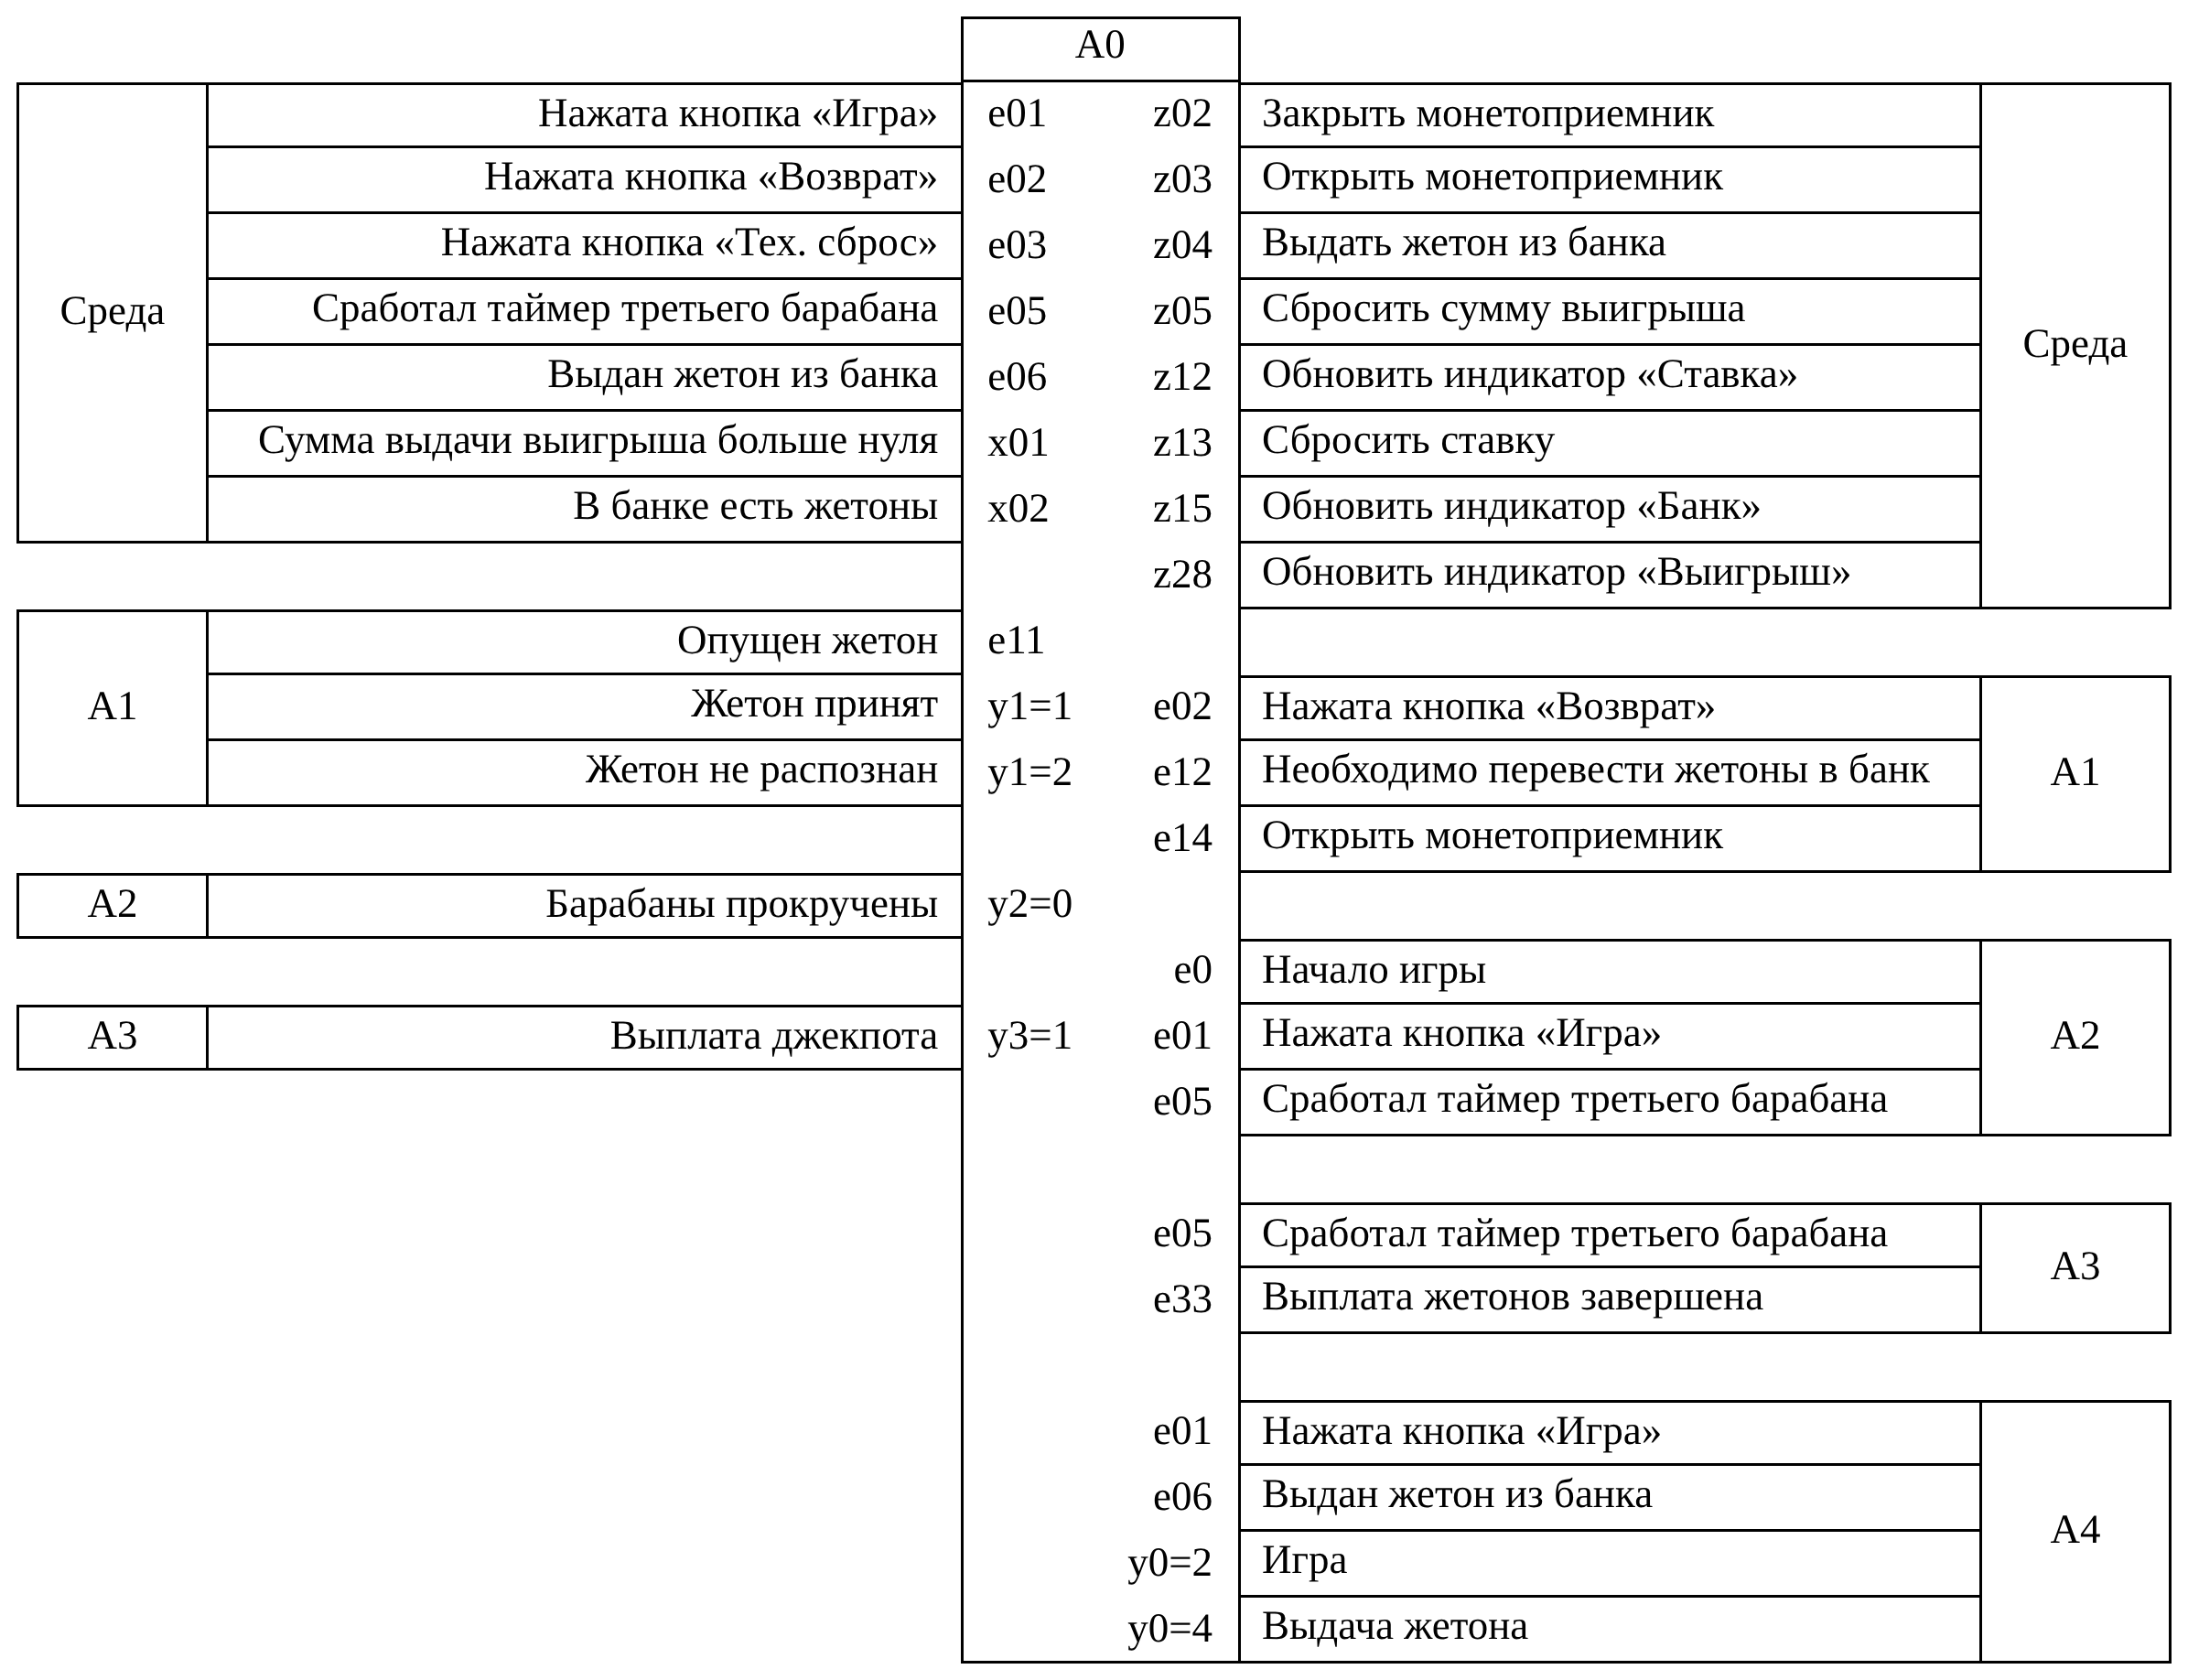
\includegraphics[width=16.50cm]{media/if_a0.png}\end{center}
% @new like=79
Рис. 1. Схема связей автомата «Игровая машина» ($A_{0}$)
% @comment: Замечания 1.11 и 1.15: интерфейс задан схемой связей, как в предыдущей работе; схема связей вставлена перед диаграммой состояний, таблица удалена. Диаграммы не менялись, изменились только номера рисунков.

% @img 78
\begin{center}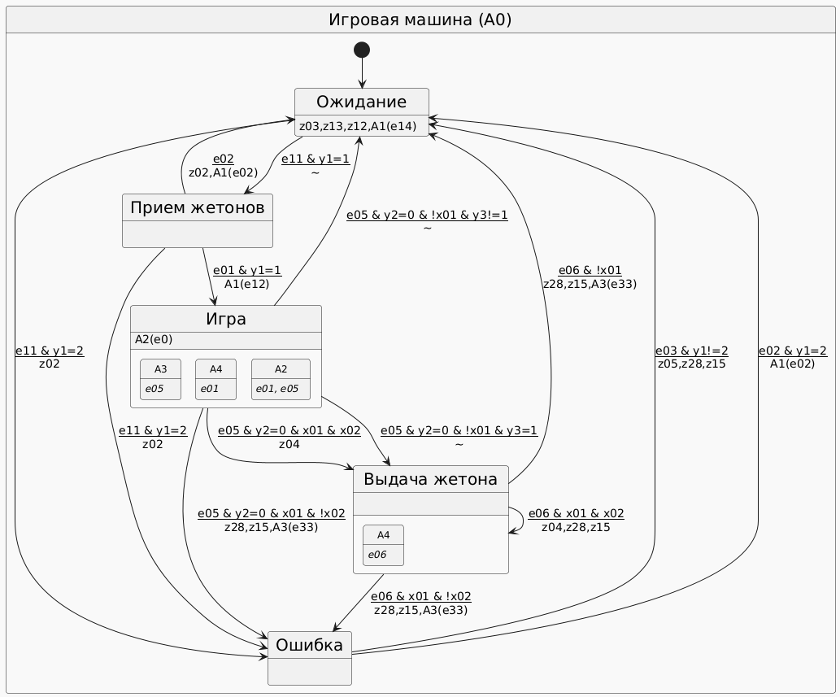
\includegraphics[width=0.8\linewidth]{media/image5.png}\end{center}
% @p 79
Рис. 2. Диаграмма состояний автомата $A_{0}$. В состояние «Игра» вложены автоматы $A_{2}$, $A_{3}$ и $A_{4}$, в состояние «Выдача жетона» – автомат $A_{4}$


% @p 93
\subsection*{Автомат 2. «Монетоприемник» ($A_{1}$)}
% @newimg like=94
\begin{center}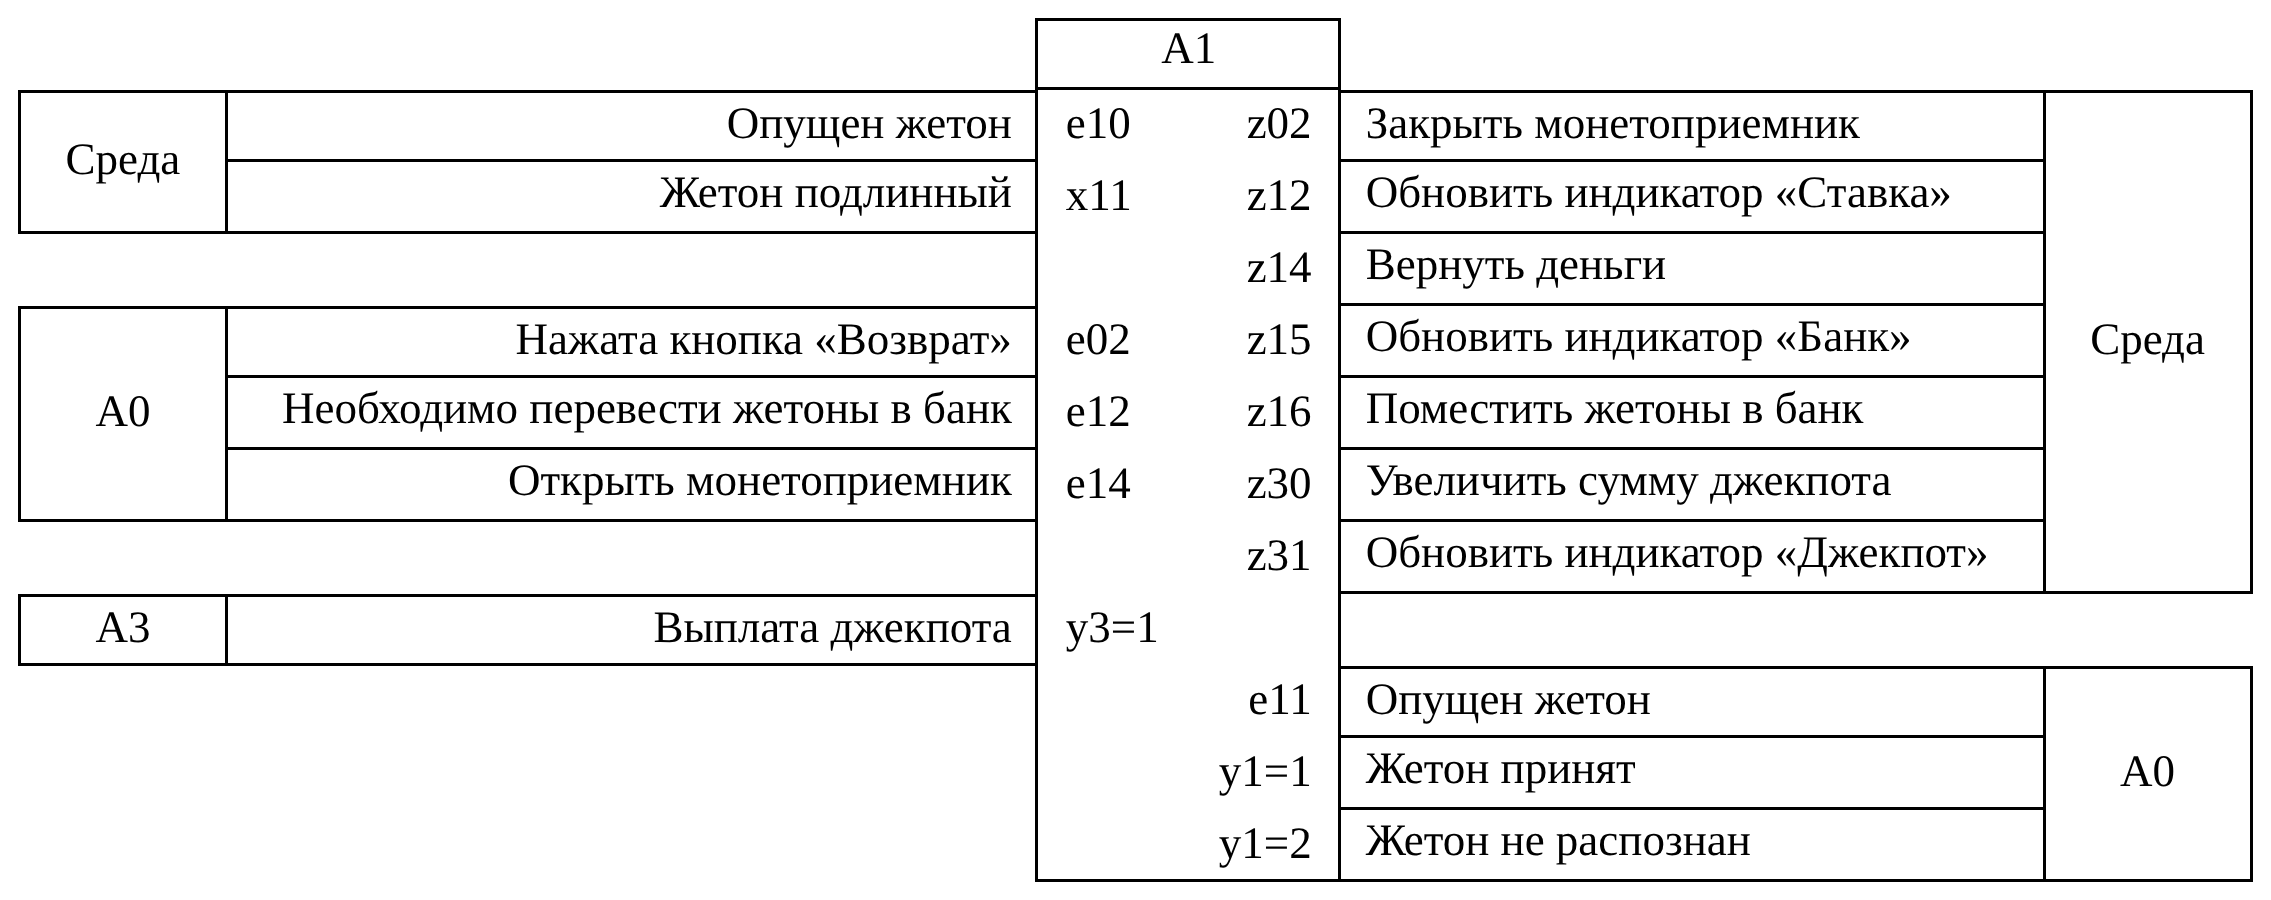
\includegraphics[width=15.67cm]{media/if_a1.png}\end{center}
% @new like=95
Рис. 3. Схема связей автомата «Монетоприемник» ($A_{1}$)

% @img 94
\begin{center}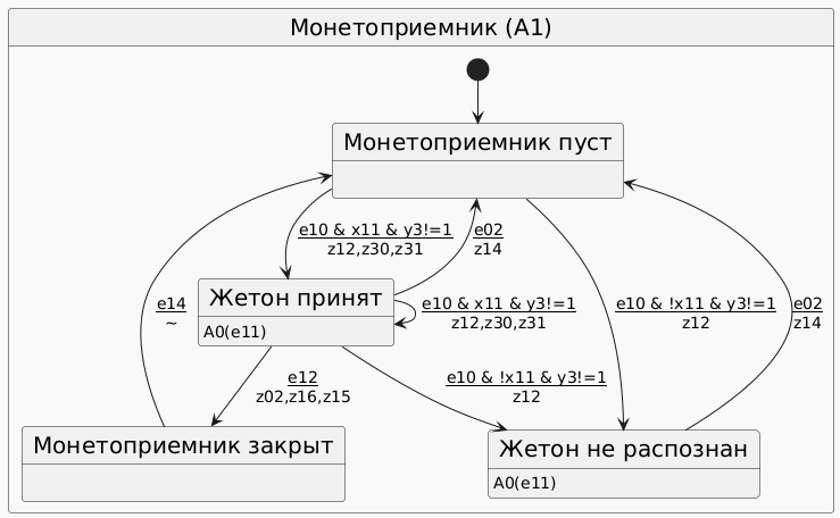
\includegraphics[width=0.8\linewidth]{media/image3.png}\end{center}
% @p 95
Рис. 4. Диаграмма состояний автомата $A_{1}$


% @p 104
\subsection*{Автомат 3. «Игровые барабаны» ($A_{2}$)}
% @newimg like=105
\begin{center}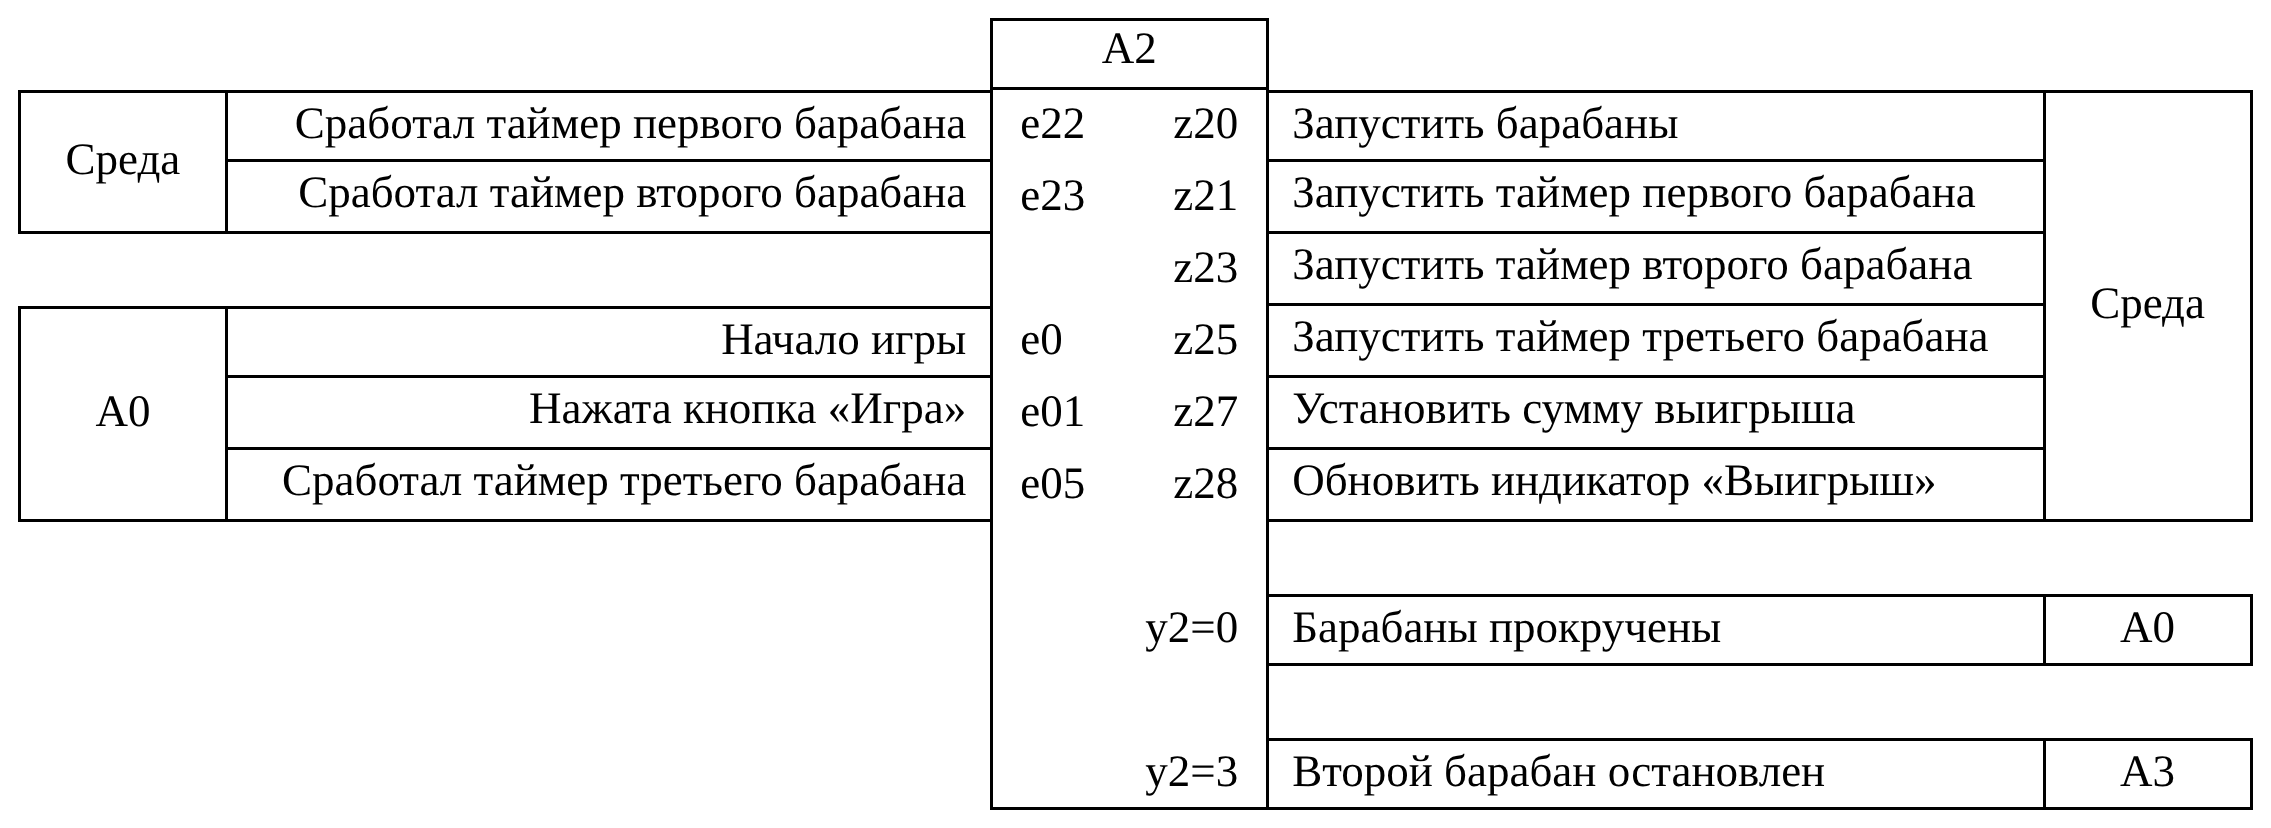
\includegraphics[width=15.67cm]{media/if_a2.png}\end{center}
% @new like=106
Рис. 5. Схема связей автомата «Игровые барабаны» ($A_{2}$)

% @img 105
\begin{center}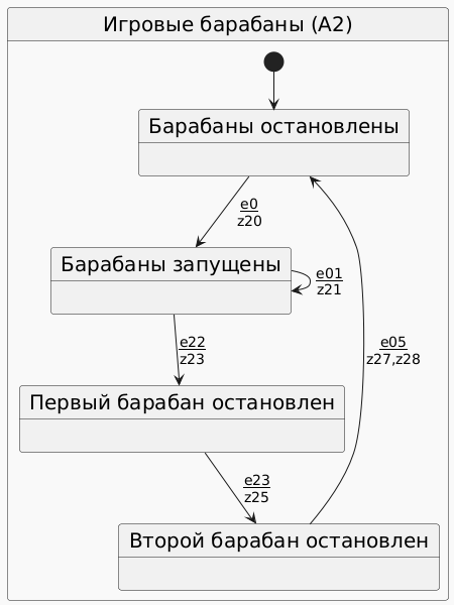
\includegraphics[width=0.8\linewidth]{media/image4.png}\end{center}
% @p 106
Рис. 6. Диаграмма состояний автомата $A_{2}$


% @p 117
\subsection*{Автомат 4. «Джекпот-счётчик» ($A_{3}$)}
% @newimg like=118
\begin{center}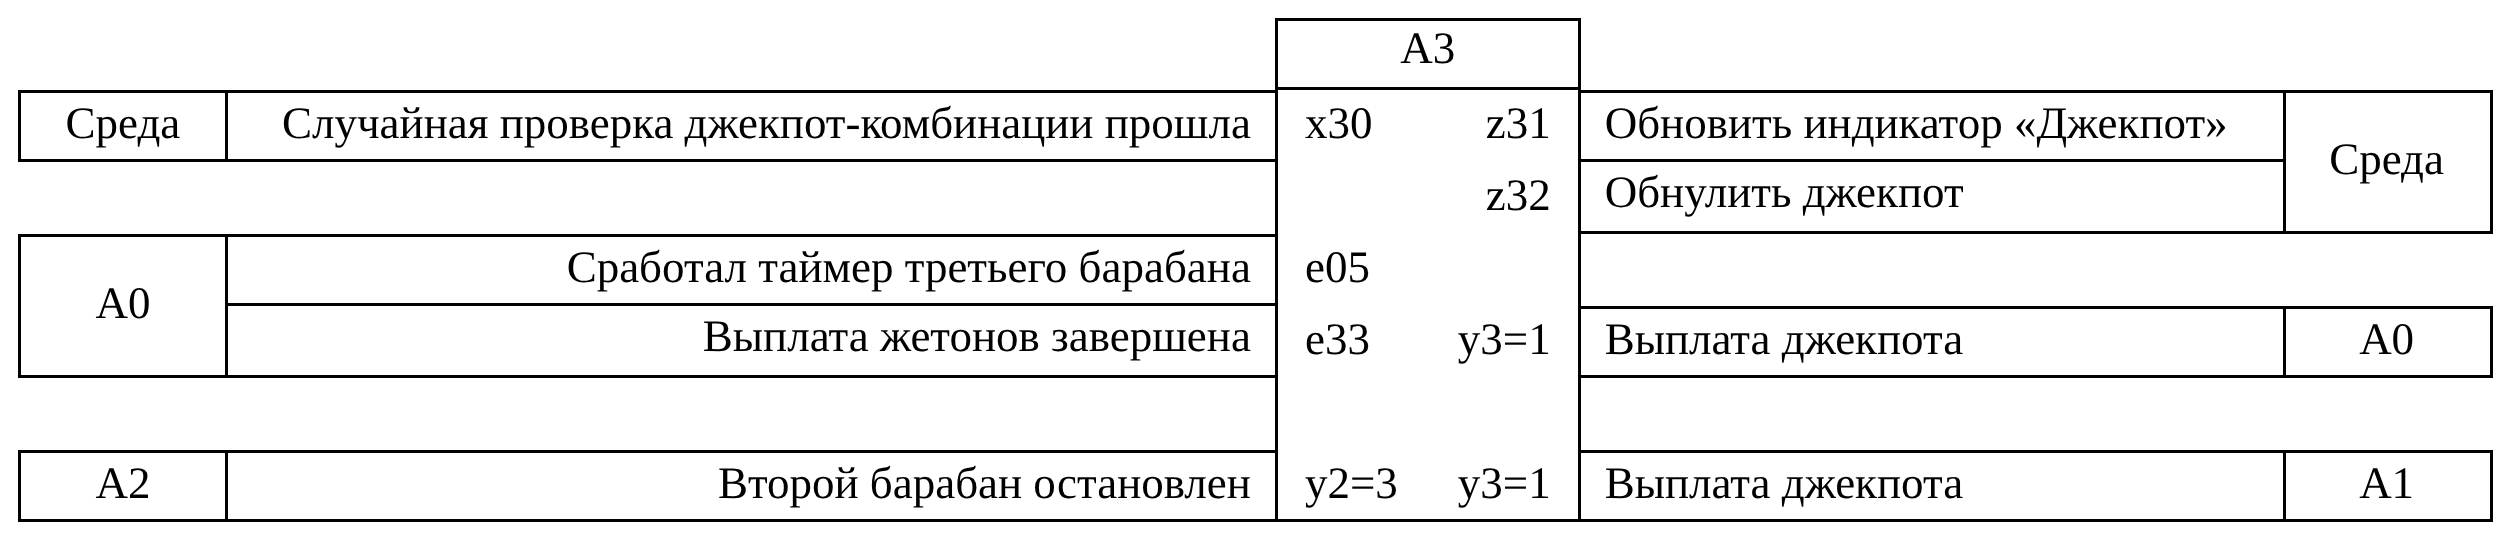
\includegraphics[width=16.50cm]{media/if_a3.png}\end{center}
% @new like=119
Рис. 7. Схема связей автомата «Джекпот-счётчик» ($A_{3}$)

% @img 118
\begin{center}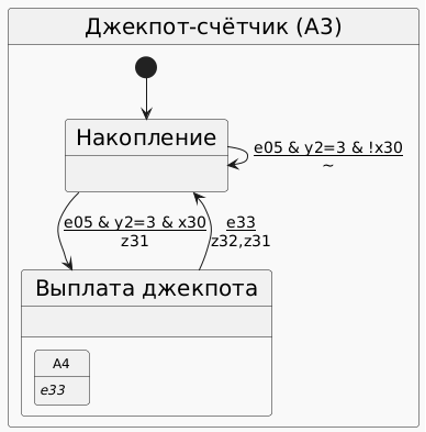
\includegraphics[width=0.8\linewidth]{media/image8.png}\end{center}
% @p 119
Рис. 8. Диаграмма состояний автомата $A_{3}$. В состояние «Выплата джекпота» вложен автомат $A_{4}$; сам автомат $A_{3}$ вложен в состояние «Игра» автомата $A_{0}$



% @p 124
\subsection*{Автомат 5. «Звуки» ($A_{4}$)}
% @newimg like=125
\begin{center}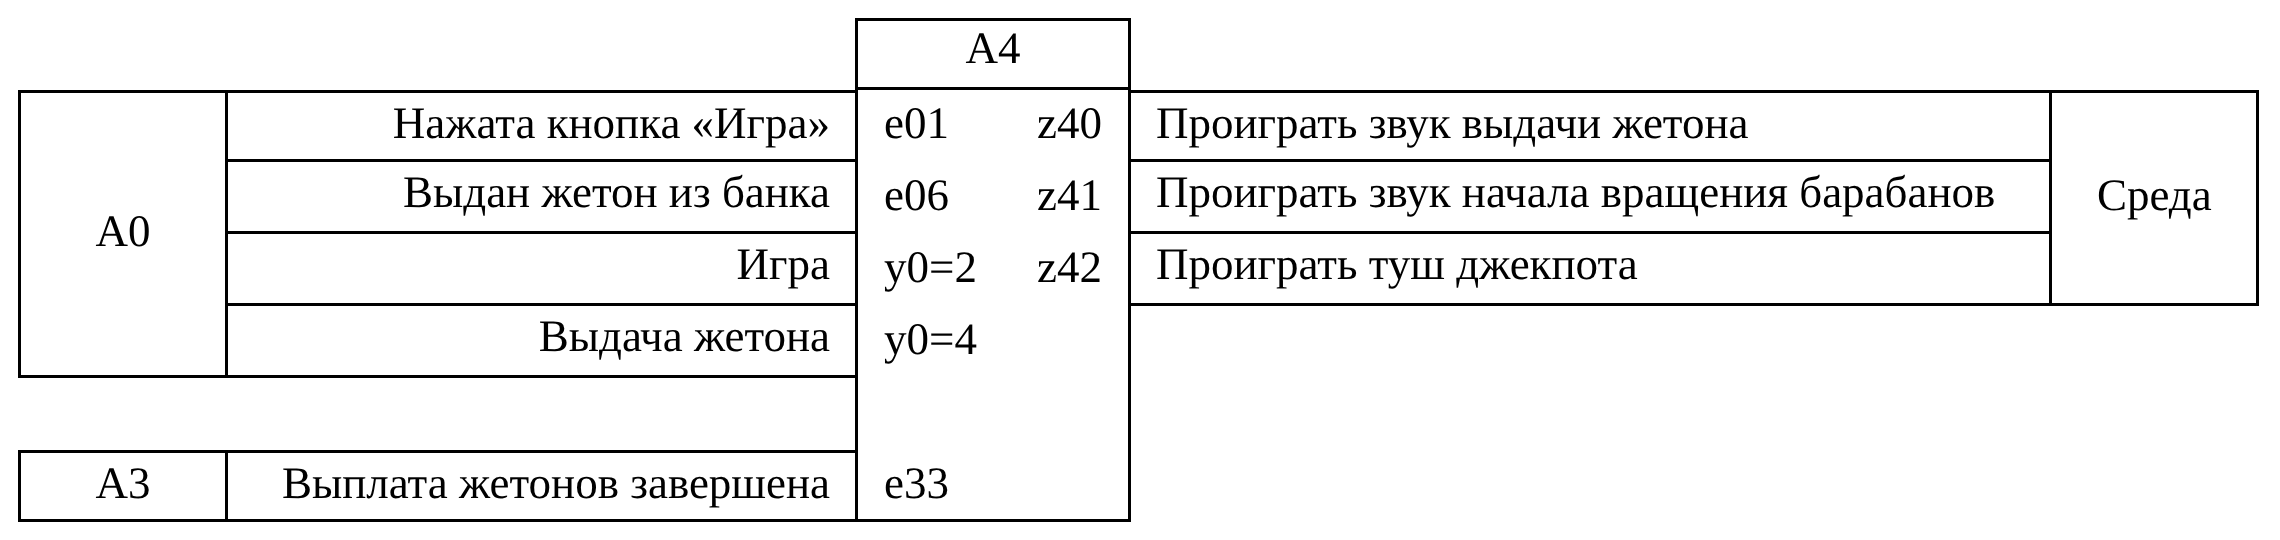
\includegraphics[width=15.73cm]{media/if_a4.png}\end{center}
% @new like=126
Рис. 9. Схема связей автомата «Звуки» ($A_{4}$)

% @img 125
\begin{center}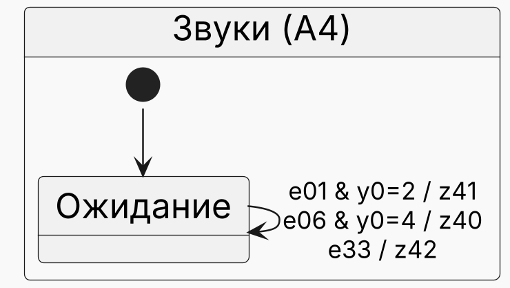
\includegraphics[width=0.8\linewidth]{media/image12.png}\end{center}
% @p 126
Рис. 10. Диаграмма состояний автомата $A_{4}$: одно состояние и петля с тремя пометками, по одной на каждое место вложения
% @new like=131
Покажем на вновь введённых автоматах $A_{3}$ (рис. 8) и $A_{4}$ (рис. 10), что в расширенной системе ограничения 1–3 сняты.
% @format: jc=both
% @comment: Замечания 1.13–1.15: текст о снятии ограничений перенесён после рисунков всех автоматов, чтобы не разрывать автоматы и схемы связей; абзац разбит по вашей правке. Абзац «Автомат A4 демонстрирует…» перенесён сюда из-под рисунка автомата A4 (1.14).
% @new like=131
Автомат $A_{3}$ вложен в состояние «Игра» автомата $A_{0}$ вместе с автоматом $A_{2}$ – в одно состояние вложено несколько автоматов (снятие ограничения 1).
% @format: jc=both
% @new like=131
Автоматы $A_{2}$ и $A_{3}$ реагируют на одно и то же событие среды e05 («Сработал таймер третьего барабана»). По этому событию автомат $A_{3}$ переходит в состояние «Выплата джекпота», если выполнен гвард из двух условий: y2=3 (второй барабан остановлен) и x30 (случайная проверка джекпот-комбинации прошла). Первое условие показывает, что автомат $A_{3}$ использует состояние автомата $A_{2}$, вложенного в то же состояние. Кроме того, это условие работает как блокировка, сдерживающая рост автомата-произведения: без него итоговый автомат содержал бы 12 состояний и 37 переходов вместо 9 и 25. Из состояния «Выплата джекпота» автомат $A_{3}$ выходит по событию e33, которое ему адресует автомат $A_{0}$ после выдачи жетонов. При этом джекпот обнуляется. Это же событие через вложенность получает и автомат $A_{4}$. Автомат $A_{4}$ демонстрирует снятие ограничений 2 и 3. Он вложен в три состояния (снятие ограничения 2), и одно из них принадлежит автомату $A_{3}$, который сам вложен в автомат $A_{0}$ (снятие ограничения 3).
% @format: jc=both
% @comment: Замечание 1.14: «Оба (какие?)» → «Автоматы A2 и A3»; «;» → «. При этом». Замечание *: выделены блокировки. Проверил на модели: без условия y2=3 итоговый автомат вырастает с 9 до 12 состояний (с 25 до 37 переходов) – это блокировка, сдерживающая рост; без условий y0=2 и y0=4 в автомате A4 состояний столько же, но переходов 30 вместо 25. Условие y3!=1 в автомате A1 (блокировка приёма жетонов во время выплаты джекпота) на размер произведения не влияет – оно нужно по смыслу.
% @new like=131
Два самоперехода (перехода из состояния в само себя) автомата $A_{4}$ – по событиям e01 (нажатие кнопки «Игра») и e06 (выдача жетона) – вызываются событиями среды, на которые реагирует и автомат $A_{0}$. Метод проверяет только, вложен ли автомат $A_{4}$ в текущее состояние автомата-произведения, но не различает, в какое из трёх состояний («Игра» или «Выдача жетона» автомата $A_{0}$, «Выплата джекпота» автомата $A_{3}$) он вложен. Поэтому без дополнительных условий автомат $A_{4}$ реагировал бы на событие e06 и в состоянии «Игра», где автомат $A_{0}$ на это событие не реагирует. Чтобы этого не было, самопереходы проверяют условия y0=2 и y0=4: реакция на событие e01 возможна только в состоянии «Игра» автомата $A_{0}$, а реакция на событие e06 – только в состоянии «Выдача жетона» того же автомата. Эти условия также сдерживают рост автомата-произведения: без них в нём было бы 30 переходов вместо 25.
% @format: jc=both
% @comment: Замечания 2.1–2.5: по вашей правке. 2.1: «через какое из мест вложения» → «в какое из трёх состояний (…) он вложен» с перечислением состояний. 2.3: «в само себя» (состояние – средний род). 2.4 («Чтобы этого не было, самопереходы») – совпадает с текущим текстом, изменений нет.
% @new like=132
Третий самопереход – по событию e33 – дополнительного условия не требует. Событие e33 адресовано автоматом $A_{0}$ автомату $A_{3}$, а автомат $A_{4}$ получает его через вложенность, только когда автомат $A_{3}$ находится в состоянии «Выплата джекпота». Поэтому автомат $A_{4}$ реагирует на событие e33 одновременно с переходом, которым автомат $A_{3}$ выходит из этого состояния (см. доработку 4 в разделе «Доработки метода»).
% @format: jc=both
% @comment: Замечание 2.6: «на e33» → «на событие e33».





% @p 134
\subsection*{Доработки метода}

% @p 135
\subsection*{Доработка 1}
% @format: before=240

% @p 136
Было. Гвард, который ссылается на состояние другого автомата, проверялся по номеру состояния этого автомата в автомате-произведении, полученном на предыдущих шагах перемножения.

% @p 137
Что ограничивало. При перемножении два состояния объединяются в одно, и номер состояния произведения перестаёт однозначно указывать состояние каждого исходного автомата. Поэтому гвард, ссылающийся на автомат, который уже вошёл в произведение, нельзя было проверить корректно. Из-за этого в состояние можно было вложить только один автомат (ограничение 1): при двух вложенных автоматах гварды, которые различают их состояния, переставали работать. По той же причине автомат нельзя было вложить больше чем в одно состояние (ограничение 2).

% @p 138
Как исправили. Теперь для каждого состояния произведения хранятся сведения о том, в каком состоянии находится каждый автомат, вошедший в произведение. При объединении состояний эти сведения объединяются, и поэтому они не теряются при перемножении цепочки автоматов. Гвард проверяется по этим сведениям и работает при любом числе автоматов, вложенных в одно состояние (ограничение 1), и при любом числе состояний, в которые вложен один автомат (ограничение 2).
% @comment: Замечания 2.7–2.8: ваша правка внесена с двумя исправлениями. «Хранится сведения» → «хранятся сведения» (согласование). «Каждый вложенный в него автомат» → «каждый автомат, вошедший в произведение»: сведения хранятся для всех перемноженных автоматов, в том числе для невложенных A0 и A1 (гвард автомата A0 проверяет состояние автомата A1, y1=1).

% @p 139
\subsection*{Доработка 2}
% @format: before=240

% @p 140
Было. Каждое состояние произведения хранит список автоматов, вложенных в него, – тех автоматов, которые в этом состоянии реагируют на события. Для нового состояния этот список составлялся просто: списки двух перемножаемых автоматов объединялись. Сначала в новый список записывались автоматы из списка первого автомата, затем – из списка второго. Повторы и автоматы, которые уже вошли в произведение, отбрасывались. Например, при умножении произведения $A_{0}$ * $A_{1}$ * $A_{2}$ на автомат $A_{3}$ состояние «Выдача жетона» автомата $A_{0}$ даёт список из автомата $A_{4}$, и состояние «Выплата джекпота» автомата $A_{3}$ – тоже из автомата $A_{4}$. Поэтому состояние произведения, в котором автоматы находятся в этих двух состояниях, получает список из одного автомата $A_{4}$. Порядок автоматов в списке важен: в этом порядке вложенные автоматы реагируют на общее событие. Так, в состоянии «Игра» автомата $A_{0}$ автомат $A_{3}$ указан раньше автомата $A_{2}$, потому что по событию e05 автомат $A_{3}$ проверяет условие y2=3 до того, как автомат $A_{2}$ по этому же событию перейдёт в другое состояние.
% @comment: Замечания 2.9 и 2.11: в текст добавлено, как объединяются списки, в каком порядке и почему порядок важен, с примерами из системы (по программе, Multiplier.kt). После «него» поставлена запятая перед тире: причастный оборот закрывается запятой.

% @p 141
Что ограничивало. Такой способ верен, пока вложенные автоматы есть только у одного из двух перемножаемых автоматов (ограничение 3). Если же вложенный автомат сам содержит вложенный автомат, способ даёт ошибку. Рассмотрим цепочку из системы: автомат $A_{3}$ вложен в состояние «Игра» автомата $A_{0}$, а автомат $A_{4}$ вложен в состояние «Выплата джекпота» автомата $A_{3}$. Через это вложение автомат $A_{4}$ должен реагировать на события, только когда выполнены два условия: автомат $A_{3}$ находится в состоянии «Выплата джекпота», а автомат $A_{0}$ – в состоянии «Игра», потому что иначе не реагирует сам автомат $A_{3}$. Простое объединение списков проверяло только первое условие. Поэтому автомат $A_{4}$ считался вложенным при любом состоянии автомата $A_{0}$, если автомат $A_{3}$ оставался в состоянии «Выплата джекпота».

% @p 142
Как исправили. Теперь список вложенного автомата добавляется в состояние произведения, только когда этот автомат сам может реагировать – его родительский автомат находится в состоянии, в которое он вложен. В примере автомат $A_{4}$ попадает в список, только если автомат $A_{3}$ находится в состоянии «Выплата джекпота», а автомат $A_{0}$ – в состоянии «Игра». Если перемножаемые автоматы не вложены друг в друга, их списки, как и раньше, объединяются. Например, автомат $A_{1}$ не вложен в автомат $A_{0}$, поэтому при умножении автомата $A_{0}$ на автомат $A_{1}$ состояние произведения, в котором автомат $A_{0}$ находится в состоянии «Игра», а автомат $A_{1}$ – в состоянии «Монетоприемник закрыт», получает список автоматов $A_{3}$, $A_{4}$ и $A_{2}$ из состояния «Игра»: у состояния «Монетоприемник закрыт» список пуст.
% @comment: Замечания 2.10 и 2.12: тире вместо «то есть», «просто» удалено, добавлен пример.

% @p 143
\subsection*{Доработка 3}
% @format: before=240
% @comment: Замечание 2.13: перед заголовком добавлен отступ 12 пт; для единообразия так же у остальных заголовков доработок и замечаний.

% @p 144
Было. Если автомат вложен в текущее состояние, то на этапе 3 любое адресованное ему событие считалось способным само по себе вызвать переход в автомате-произведении, так же, как событие среды.
% @comment: Замечание 2.13: добавлено «то».

% @p 145
Что ограничивало. Адресованное событие возникает только в момент перехода автомата-отправителя. Поэтому, рассматривая его отдельно от этого перехода, метод строил переходы, которых нет в исходной системе. В рассматриваемой системе это проявилось при вложении автомата $A_{4}$ в автомат $A_{3}$ (ограничение 3): в автомате-произведении был переход, в котором автомат $A_{4}$ воспроизводил звуковой сигнал выигрыша джекпота (z42), а автомат $A_{3}$ оставался в состоянии «Выплата джекпота».

% @p 146
Как исправили. Теперь вложенный автомат реагирует на событие сам по себе, только если хотя бы один из автоматов, уже вошедших в произведение, объявляет это событие событием среды. Адресованное событие вложенный автомат получает только вместе с переходом автомата-отправителя.

% @p 147
\subsection*{Доработка 4}
% @format: before=240

% @p 148
Было. Адресованное событие поступало только автомату-получателю.

% @p 149
Что ограничивало. Поэтому автомат, вложенный в состояние получателя, не мог отреагировать на такое событие. В рассматриваемой системе автомат $A_{4}$ вложен в состояние «Выплата джекпота» автомата $A_{3}$, но не мог отреагировать на событие e33, по которому автомат $A_{3}$ выходит из этого состояния.

% @p 150
Как исправили. Теперь адресованное событие получает не только получатель, но и автоматы, вложенные в то состояние, в котором получатель был до перехода. Их реакции входят в тот же переход автомата-произведения. Бывает, что такой вложенный автомат ещё не вошёл в произведение: автоматы умножаются по одному, и на текущем шаге он ещё не умножен. Тогда на переходе произведения сохраняется отметка о том, что событие этому автомату не доставлено. На одном из следующих шагов, когда произведение умножается на этот автомат, отметка обрабатывается как событие, адресованное ему напрямую, и его реакция добавляется к тому же переходу. Например, при порядке $A_{0}$, $A_{1}$, $A_{2}$, $A_{3}$, $A_{4}$ событие e33 на шаге умножения на автомат $A_{3}$ запоминается для автомата $A_{4}$ и доставляется ему на шаге умножения на автомат $A_{4}$.
% @comment: Замечание 2.14 («когда автомат войдёт в произведение ???»): объяснено, что автоматы умножаются по одному, что именно запоминается и когда доставляется, добавлен пример с e33.

% @p 151
\subsection*{Замечание о порядке умножения}
% @format: before=240

% @p 152
Порядок, в котором перемножаются автоматы, важен в двух случаях, и каждый из них задаёт требование к порядку. Первый случай – гварды: если гвард автомата Y ссылается на состояние автомата X, то автомат X должен войти в произведение не позднее автомата Y (требование 1). Иначе результат умножения может не совпадать с поведением исходной системы. Например, так происходит при порядке $A_{0}$, $A_{2}$, $A_{1}$, потому что автомат $A_{0}$ содержит гвард на состояние автомата $A_{1}$.
% @comment: Замечание 2.15: требования названы явно – «требование 1» и «требование 2», на них ссылаются этап 1, перечень ограничений и вывод.

% @p 153
Для адресованных событий требование зависит от того, как событие доставляется. Если получатель получает событие напрямую, порядок не важен. Раньше, если отправитель ещё не вошёл в произведение, получатель реагировал на его событие так, будто оно может возникнуть в любой момент, и появлялись лишние состояния. Теперь получатель не реагирует на такое событие, пока отправитель не войдёт в произведение.

% @p 154
Второй случай, когда порядок важен, – события, которые приходят через вложенность (доработка 4): вложенный автомат должен войти в произведение после родительского (требование 2). Иначе в момент доставки события родительскому автомату вложенный автомат уже входит в произведение, переход не запоминает недоставленное событие, и реакция вложенного автомата теряется. Поэтому в рассматриваемой системе автомат $A_{4}$ умножается после автомата $A_{3}$, а при порядке $A_{0}$, $A_{1}$, $A_{2}$, $A_{4}$, $A_{3}$ программа сообщает об ошибке.

% @p 155
Оба требования можно проверить по виду перемножаемых автоматов до перемножения: требование 1 – по гвардам, требование 2 – по вложенности. Поэтому отдельный этап для выбора порядка не нужен: порядок выбирают на этапе 1 так, чтобы оба требования выполнялись. Если на этапе 7 поведение автомата-произведения и исходной системы всё же различается, то порядок перемножения автоматов меняют вручную и перемножение повторяют. Предметом дальнейшей работы остаётся другое: как доработать метод так, чтобы требования 1 и 2 стали не нужны и подходил любой порядок перемножения.
% @comment: Замечания 2.15 и 2.20: в текст добавлено, что делать сейчас (выбрать порядок на этапе 1 по требованиям, при расхождении на этапе 7 поменять порядок вручную), почему отдельный этап не нужен и что именно остаётся дальнейшей работой.

% @p 156
\subsection*{Замечание об обратном вызове}
% @format: before=240

% @p 157
Как и в предыдущей работе [1], обратный вызов не допускается. Обратный вызов – это случай, когда автомат A на своём переходе адресует событие автомату B, а автомат B в ответ адресует событие автомату A. Метод такую ответную реакцию не строит: в автомате-произведении автомат A на неё не реагирует. Расхождение с исходной системой при этом обнаруживается на этапе 7, что проверено на паре автоматов с обратным вызовом.

% @p 158
\subsection*{Замечание о моменте первой реакции вложенного автомата}
% @format: before=240

% @p 159
Вложенность проверяется по состоянию родительского автомата до перехода. Поэтому автомат, вложенный в целевое состояние перехода, не реагирует на событие, которое вызвало этот переход: он начинает реагировать только на следующие события. Если реакция нужна сразу при входе в состояние, её передают адресованным событием. Так, автомат $A_{0}$ при входе в состояние «Игра» адресует автомату $A_{2}$ событие e0 («Начало игры»). Чтобы снять это ограничение, метод должен при построении перехода опрашивать автоматы, вложенные в его целевое состояние, хотя это состояние в автомате-произведении ещё не построено. Это требует существенно изменить устройство метода и остаётся предметом дальнейшей работы.
% @new like=158
Ограничения доработанного подхода
% @format: before=240
% @comment: Замечания 2.16–2.17 и вопрос о классе задач: новый раздел – перечень ограничений, которые остаются после доработки, и класс задач, решаемых подходом при этих ограничениях. Пункт 4 – то, что показано на автомате A4.
% @new like=159
После доработки у подхода остаются следующие ограничения. При их нарушении автомат-произведение может функционировать не так, как исходная система, и метод применять не следует.
% @new like=159
1. Порядок перемножения автоматов должен удовлетворять требованиям 1 и 2 (раздел «Замечание о порядке умножения»).
% @new like=159
2. Обратный вызов не допускается (раздел «Замечание об обратном вызове»).
% @new like=159
3. Вложенный автомат не реагирует на событие, которое переводит родительский автомат в состояние, куда он вложен. Если реакция нужна сразу при входе в состояние, её передают адресованным событием (раздел «Замечание о моменте первой реакции вложенного автомата»).
% @new like=159
4. Метод не различает, через какое из мест вложения автомат вложен в текущее состояние произведения. Если реакции вложенного автомата должны зависеть от места вложения, это задают гвардами на состояние родительского автомата, как в автомате $A_{4}$.
% @new like=159
При этих ограничениях подход применим к системам взаимодействующих автоматов, в которых вложенность может иметь любую глубину, в одно состояние может быть вложено несколько автоматов, а один автомат может быть вложен в несколько состояний. Автоматы взаимодействуют через проверку состояний друг друга и адресованные события без обратного вызова, и для них существует порядок перемножения, удовлетворяющий требованиям 1 и 2. К таким системам относятся, например, системы логического управления устройствами, в которых режимы работы задаются состояниями управляющего автомата, а в каждом режиме работают свои подчинённые автоматы, как в рассматриваемой системе «игровой автомат».

% @p 174
\subsection*{Итоговый перемноженный автомат}
% @newimg like=175
\begin{center}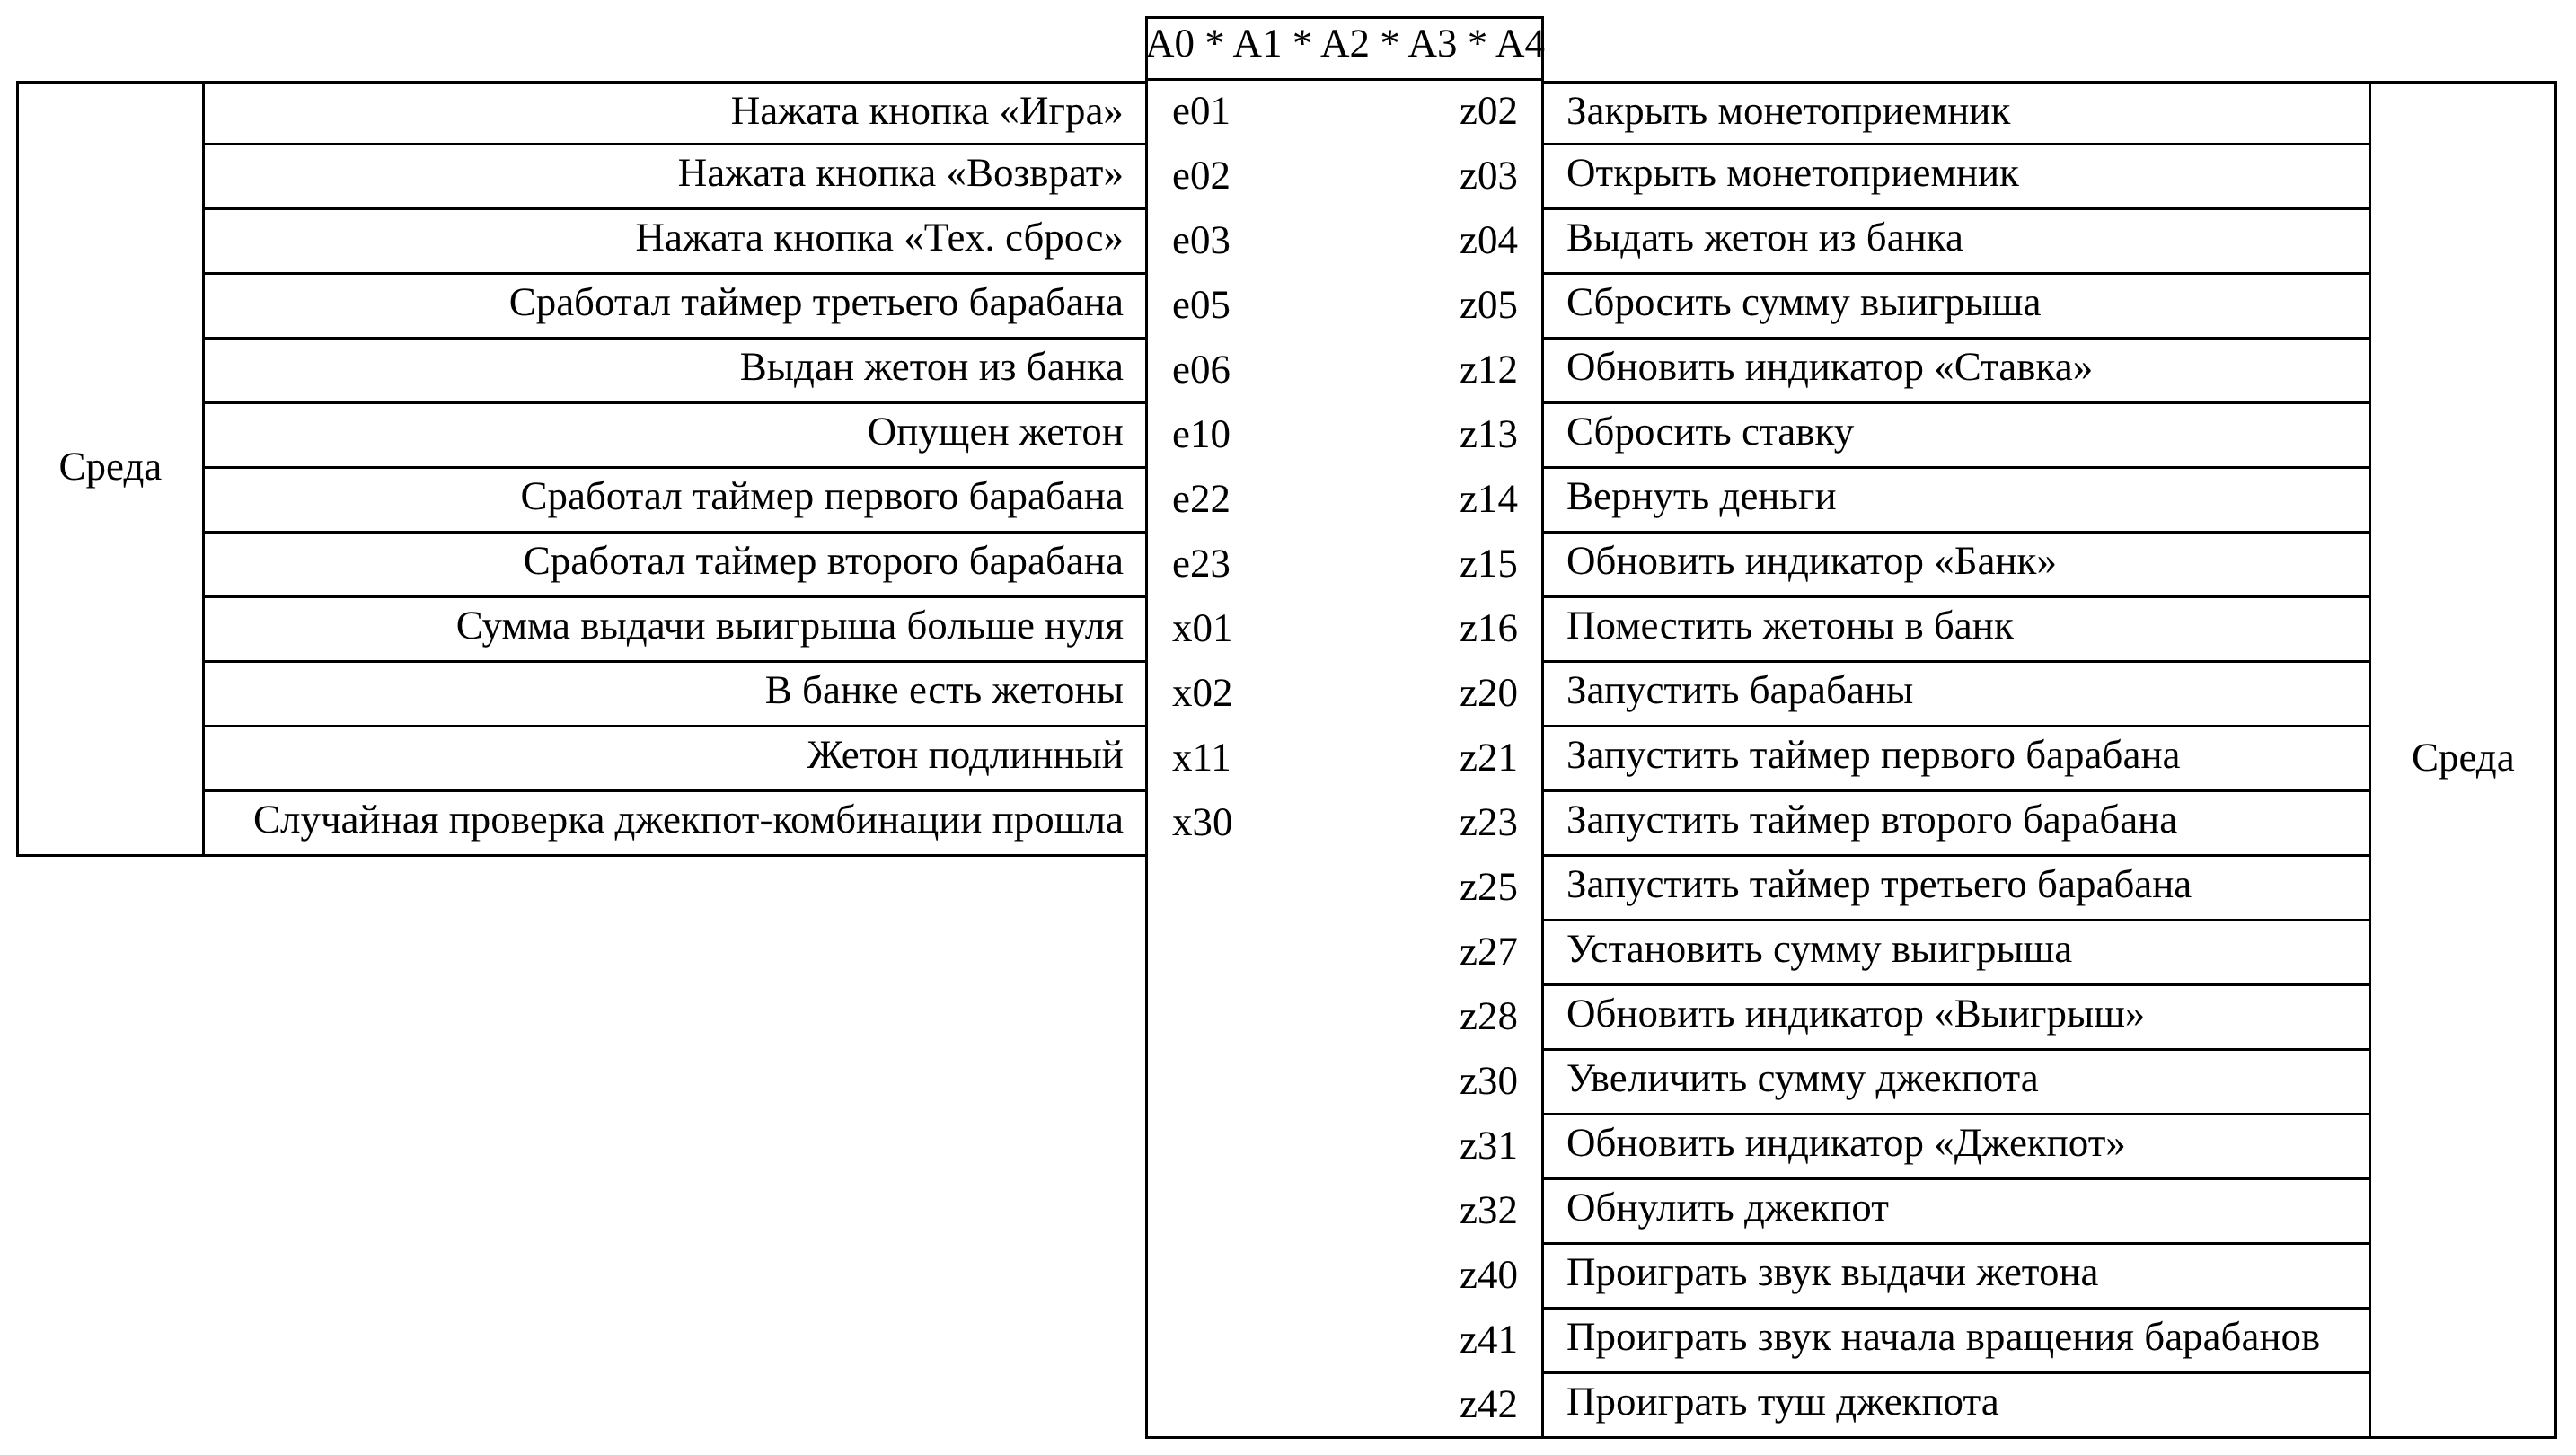
\includegraphics[width=16.50cm]{media/if_final.png}\end{center}
% @new like=176
Рис. 11. Схема связей итогового автомата $A_{0}$ * $A_{1}$ * $A_{2}$ * $A_{3}$ * $A_{4}$
% @comment: Замечания 1.11 и 1.15: схема связей итогового автомата вставлена перед его диаграммой, таблица 7 удалена.

% @img 175
\begin{center}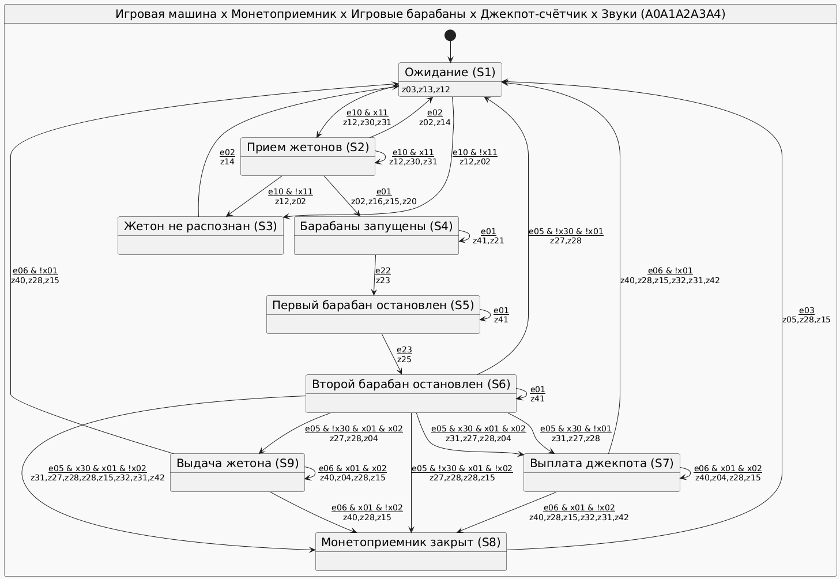
\includegraphics[width=0.8\linewidth]{media/image2.png}\end{center}
% @p 176
Рис. 12. Диаграмма состояний итогового автомата $A_{0}$*$A_{1}$*$A_{2}$*$A_{3}$*$A_{4}$ (9 состояний). 

% @p 177
Состояния подписаны сокращёнными названиями; соответствие каждого состояния исходным состояниям пяти автоматов приведено ниже

% @p 178
S1 – $A_{0}$: Ожидание, $A_{1}$: Монетоприемник пуст, $A_{2}$: Барабаны остановлены, $A_{3}$: Накопление, $A_{4}$: Ожидание

% @p 179
S2 – $A_{0}$: Прием жетонов, $A_{1}$: Жетон принят, $A_{2}$: Барабаны остановлены, $A_{3}$: Накопление, $A_{4}$: Ожидание

% @p 180
S3 – $A_{0}$: Ошибка, $A_{1}$: Жетон не распознан, $A_{2}$: Барабаны остановлены, $A_{3}$: Накопление, $A_{4}$: Ожидание

% @p 181
S4 – $A_{0}$: Игра, $A_{1}$: Монетоприемник закрыт, $A_{2}$: Барабаны запущены, $A_{3}$: Накопление, $A_{4}$: Ожидание

% @p 182
S5 – $A_{0}$: Игра, $A_{1}$: Монетоприемник закрыт, $A_{2}$: Первый барабан остановлен, $A_{3}$: Накопление, $A_{4}$: Ожидание

% @p 183
S6 – $A_{0}$: Игра, $A_{1}$: Монетоприемник закрыт, $A_{2}$: Второй барабан остановлен, $A_{3}$: Накопление, $A_{4}$: Ожидание

% @p 184
S7 – $A_{0}$: Выдача жетона, $A_{1}$: Монетоприемник закрыт, $A_{2}$: Барабаны остановлены, $A_{3}$: Выплата джекпота, $A_{4}$: Ожидание

% @p 185
S8 – $A_{0}$: Ошибка, $A_{1}$: Монетоприемник закрыт, $A_{2}$: Барабаны остановлены, $A_{3}$: Накопление, $A_{4}$: Ожидание

% @p 186
S9 – $A_{0}$: Выдача жетона, $A_{1}$: Монетоприемник закрыт, $A_{2}$: Барабаны остановлены, $A_{3}$: Накопление, $A_{4}$: Ожидание


% @p 191
\subsection*{Вывод}

% @p 192
Предложенные доработки снимают три ограничения предыдущей работы. Теперь в состояние можно вложить несколько автоматов (ограничение 1), автомат можно вложить в несколько состояний (ограничение 2), а вложенные автоматы могут содержать оба перемножаемых автомата (ограничение 3). Вместе это позволяет строить цепочки вложенности любой глубины. Кроме того, исправлена ошибка, при которой вложенный автомат реагировал на адресованное событие отдельно от перехода отправителя (доработка 3), и адресованное событие теперь получают также автоматы, вложенные в состояние получателя (доработка 4).

% @p 193
Порядок перемножения автоматов по-прежнему важен в двух случаях (требования 1 и 2). Автомат, на состояние которого ссылается гвард, должен войти в произведение не позднее автомата с этим гвардом. Автомат, который получает адресованные события через вложенность, должен войти в произведение после родительского. Для адресованных событий, которые приходят напрямую, порядок не важен. Оба требования проверяются по виду автоматов до перемножения.
% @comment: Замечание 2.20: ссылка на требования 1 и 2 и на то, что их можно проверить заранее.

% @p 194
Итоговый автомат-произведение содержит 9 состояний и 25 переходов, а исходная система из пяти автоматов – 16 состояний и 33 перехода. Верхняя оценка числа состояний произведения равна 5·4·4·2·1 = 160. Промежуточные автоматы-произведения тоже не были громоздкими: после умножения на автоматы $A_{1}$, $A_{2}$, $A_{3}$ и $A_{4}$ они содержали 6, 8, 9 и 9 состояний. Поэтому эвристическая корректировка перемножаемых автоматов (этап 5) в этом примере не понадобилась. В чём она состоит, описано в предыдущей работе [1]. Автомат-произведение и исходная система функционируют одинаково на всех последовательностях входных воздействий длиной до 20 и на 1000 случайных последовательностях длиной 100. Программа, которая реализует предлагаемый метод перемножения автоматов, опубликована по адресу https://github.com/PhoenixNazarov/fsm-multiply.
% @comment: Замечания 2.18 и 2.19: числа сопоставлены попарно (9 и 25 против 16 и 33; посчитано программой), добавлено, что корректировка не понадобилась, с размерами промежуточных произведений и ссылкой на [1].
% @new like=191
Литература
% @comment: Замечание 1.0: список литературы. Название статьи взято с сайта журнала: «Валидация…» (в замечании было «Валидации…»).
% @new like=194
1. Назаров В. А., Шалыто А. А. Валидация автоматных спецификаций на основе перемножения автоматов // Информационно-управляющие системы. 2026. № 5. С. 21–36. doi:10.31799/1684-8853-2026-5-21-36

\end{document}
